\documentclass[11pt,a4paper]{article}
\usepackage{kotex}
\usepackage{amsmath,amssymb,amsfonts,amsthm}
\usepackage{graphicx}
\usepackage{booktabs}
\usepackage{algorithm}
\usepackage{algorithmic}
\usepackage{hyperref}
\usepackage{xcolor}
\usepackage{geometry}
\usepackage{tikz}
\usepackage{pgfplots}
\usetikzlibrary{shapes.geometric, arrows, positioning, fit, calc, backgrounds}
\pgfplotsset{compat=1.17}
\geometry{margin=2.5cm}

\newtheorem{theorem}{정리}
\newtheorem{lemma}{보조정리}
\newtheorem{definition}{정의}

\DeclareMathOperator*{\argmax}{arg\,max}
\DeclareMathOperator*{\argmin}{arg\,min}
\DeclareMathOperator*{\E}{\mathbb{E}}
\DeclareMathOperator*{\CVaR}{\mathrm{CVaR}}
\DeclareMathOperator*{\VaR}{\mathrm{VaR}}

\title{\textbf{STAIR-RL: 의미적 토큰 증강 정보이론적 강화학습을 통한\\암호화폐 포트폴리오 관리}}
\author{프로젝트 보고서}
\date{2025년 12월}

\begin{document}

\maketitle

\begin{abstract}
본 프로젝트는 STAIR-RL (Semantic Token-Augmented Information-theoretic Reinforcement Learning) 프레임워크를 구현하고 분석한다.
STAIR-RL은 대규모 언어 모델(LLM)의 의미적 토큰을 전통적인 수치 특징과 결합하여 암호화폐 포트폴리오 관리를 위한 강화학습 에이전트를 학습한다.
핵심 기여는 다음과 같다: (1) 정보이론적 기반의 토큰 선택 메커니즘인 TERC (Transfer Entropy Relevance Criterion), (2) 동적 의미 게이팅을 통한 노이즈 필터링, (3) CQL-SAC에서 PPO-CVaR로의 2단계 오프라인-온라인 전이 학습, (4) CVaR 제약을 통한 테일 리스크 관리.
본 보고서에서는 POMDP 정식화, Late Fusion 아키텍처, 정보이론적 분석, 그리고 구현 상세를 체계적으로 다룬다.
\end{abstract}

\vspace{0.5em}
\noindent\textbf{코드 저장소}: \url{https://github.com/menschhelt/STAIR-RL}

%==============================================================================
\section{서론}
%==============================================================================

\subsection{연구 배경}

2022년 Terra/Luna 붕괴와 FTX 파산 사태는 암호화폐 시장에서 테일 리스크(tail risk) 관리의 중요성을 극명하게 보여주었다.
불과 며칠 사이에 시가총액 수백억 달러가 증발했고, 이는 전통적인 위험 중립적(risk-neutral) 투자 전략의 한계를 드러냈다.

기존의 강화학습 기반 포트폴리오 관리 방법론은 이러한 극단적 상황에 대응하기 어렵다.
대부분의 RL 알고리즘이 기대 수익만을 최대화하기 때문에, 99.9\% 손실 같은 테일 이벤트는 학습 목표에 거의 영향을 미치지 않는다.
더욱이 기존 연구들은 가격과 거래량 같은 정형 데이터에만 의존하여, 규제 발표나 해킹 뉴스 같은 시장 급변의 전조를 포착하지 못한다.
암호화폐 시장의 비정상성(non-stationarity)---시장 레짐의 급격한 전환, 규제 환경의 변화, 새로운 자산군의 등장---은 오프라인에서 학습된 정책을 빠르게 무력화시킨다.

최근 대규모 언어 모델(LLM)의 발전은 이러한 한계를 극복할 새로운 가능성을 열었다.
FinBERT, CryptoBERT 같은 금융 특화 언어 모델은 뉴스와 소셜 미디어에서 시장 심리와 이벤트 정보를 추출할 수 있다.
그러나 LLM 출력을 강화학습에 \textit{효과적으로} 통합하는 방법론은 아직 체계화되지 않았으며, 단순히 임베딩을 연결하는 것만으로는 노이즈가 신호를 압도할 위험이 있다.

\subsection{핵심 연구 질문}

본 프로젝트는 다음 질문에 답한다:

\begin{quote}
\textit{``의미적 정보(semantic information)가 순차적 의사결정에 얼마나 가치가 있는가, 그리고 이를 어떻게 최적으로 활용할 것인가?''}
\end{quote}

STAIR-RL은 이 질문에 대해 정보이론적 프레임워크를 제시하며, 의미적 토큰의 가치가 조건부 상호정보량의 $\sqrt{I}$ 스케일로 증가함을 이론적으로 보인다.

\subsection{주요 기여}

\begin{enumerate}
    \item \textbf{TERC (Transfer Entropy Relevance Criterion)}: 전이 엔트로피 기반으로 행동 결정에 유용한 의미적 토큰을 선택하는 정보이론적 기준. 서브모듈러 최적화를 통해 $(1-1/e)$-근사 보장.

    \item \textbf{동적 의미 게이팅}: 수치적 시장 상태에 따라 의미적 정보의 가중치를 자동으로 조절하는 학습 가능한 게이트 메커니즘.

    \item \textbf{2단계 전이 학습}: CQL-SAC 오프라인 사전학습(36개월)에서 PPO-CVaR 온라인 미세조정(12개월)으로의 하이브리드 접근.

    \item \textbf{CVaR 제약}: 라그랑지안 쌍대 방법 기반의 테일 리스크 제어로 극단적 손실 방지.
\end{enumerate}

%==============================================================================
\section{문제 분석 및 모티베이션}
%==============================================================================

기존 RL 기반 암호화폐 트레이딩 연구의 한계를 체계적으로 분석한다.

\subsection{위험 중립성 문제 (Risk Neutrality)}

대부분의 RL 알고리즘은 다음 목적함수를 최적화한다:
\begin{equation}
\max_\pi \mathbb{E}_\pi \left[ \sum_{t=0}^{\infty} \gamma^t r_t \right]
\end{equation}

이는 수익 분포의 평균만 고려하며 분산이나 테일 리스크를 무시한다.
2022년 Terra/Luna 사태에서 99.9\% 이상 가치가 증발한 것처럼, 암호화폐 시장에서는 극단적 손실이 빈번하게 발생한다.
기대 수익 최대화는 이러한 ``블랙 스완'' 이벤트에 취약하다.

\subsection{비정상성과 분포 이동 (Non-Stationarity)}

암호화폐 시장은 다음과 같은 비정상적 특성을 보인다:
\begin{itemize}
    \item 시장 레짐(bull/bear/sideways)이 빠르게 전환
    \item 규제 환경이 급변 (중국의 채굴 금지, SEC 규제 등)
    \item 새로운 자산군의 등장 (DeFi, NFT, Meme 코인)
\end{itemize}

학습 데이터와 배포 환경 간의 분포 이동(distributional shift)으로 인해 오프라인에서 학습된 정책이 온라인 환경에서 실패할 수 있다.

\subsection{가짜 상관관계 (Spurious Correlations)}

고차원 특징 공간에서 RL 에이전트는 다음과 같은 가짜 상관관계를 학습할 수 있다:
\begin{itemize}
    \item 특정 시간대에만 유효한 패턴 (예: 주말 효과)
    \item 소수 이벤트에 과적합 (예: FTX 붕괴 직전 패턴)
    \item 우연히 수익과 상관된 무관한 특징
\end{itemize}

의미적 정보는 인과관계에 더 가까운 정보를 제공하여 이러한 가짜 상관관계를 완화할 수 있다.

\subsection{LLM 활용의 기술적 과제}

LLM을 실시간 트레이딩에 적용할 때 다음 과제가 발생한다:

\begin{itemize}
    \item \textbf{추론 지연}: GPT-4 수준 모델의 추론 시간(수 초)은 5분봉 트레이딩에도 부담
    \item \textbf{감성 불일치}: 언어적 감성(positive/negative)과 금융적 함의가 다를 수 있음
    \item \textbf{정보 과잉}: 모든 토큰이 트레이딩에 유용한 것은 아님
\end{itemize}

STAIR-RL은 사전 계산된 임베딩과 정보이론적 토큰 선택으로 이 문제들을 해결한다.

%==============================================================================
\section{문제 정식화: POMDP}
%==============================================================================

\subsection{부분 관측 마르코프 결정 과정}

암호화폐 포트폴리오 관리 문제를 POMDP로 정식화한다:

\begin{definition}[POMDP]
POMDP $\mathcal{M} = (\mathcal{S}, \mathcal{A}, \mathcal{O}, \mathcal{T}, \mathcal{Z}, r, \gamma)$는 다음으로 구성된다:
\begin{itemize}
    \item $\mathcal{S}$: 상태 공간 (잠재 시장 레짐 포함)
    \item $\mathcal{A} = [-1, 1]^N$: 행동 공간 (N개 자산의 포트폴리오 가중치)
    \item $\mathcal{O}$: 관측 공간 (수치적 특징 + 의미적 토큰)
    \item $\mathcal{T}: \mathcal{S} \times \mathcal{A} \rightarrow \Delta(\mathcal{S})$: 전이 확률
    \item $\mathcal{Z}: \mathcal{S} \rightarrow \Delta(\mathcal{O})$: 관측 확률
    \item $r: \mathcal{S} \times \mathcal{A} \rightarrow \mathbb{R}$: 보상 함수 (로그 수익률 - 거래비용)
    \item $\gamma \in (0, 1)$: 할인율
\end{itemize}
\end{definition}

\subsection{부분 관측 문제}

에이전트는 진정한 상태 $s_t$를 직접 관측할 수 없다.
진정한 상태에는 다음이 포함된다:
\begin{itemize}
    \item 현재 시장 레짐 (상승장/하락장/횡보장)
    \item 다른 참여자들의 포지션과 의도
    \item 미공개 정보 (내부자 거래, 규제 계획 등)
\end{itemize}

에이전트가 관측하는 것은 $o_t = (F_t, H_t, x_t^{\text{port}})$로 구성된다:
\begin{itemize}
    \item $F_t \in \mathbb{R}^{N \times d_F}$: 수치적 팩터 (Alpha 101)
    \item $H_t \in \mathbb{R}^{d_H}$: 의미적 임베딩 (FinBERT, CryptoBERT)
    \item $x_t^{\text{port}} \in \mathbb{R}^{N+2}$: 현재 포트폴리오 상태
\end{itemize}

\subsection{CVaR 제약 목적함수}

기대 수익 최대화에 리스크 제약을 추가한다:

\begin{equation}
\max_\pi \mathbb{E}_\pi \left[ \sum_{t=0}^{\infty} \gamma^t r_t \right] \quad \text{s.t.} \quad \text{CVaR}_\alpha(-R) \leq \kappa
\end{equation}

여기서 $\text{CVaR}_\alpha(-R)$는 손실의 $\alpha$-분위수 초과 조건부 기대값이다:
\begin{equation}
\text{CVaR}_\alpha(-R) = \mathbb{E}[-R \mid -R \geq \text{VaR}_\alpha(-R)]
\end{equation}

라그랑지안 쌍대 문제로 변환하면:
\begin{equation}
\min_{\lambda \geq 0} \max_\pi \mathcal{L}(\pi, \lambda) = \mathbb{E}_\pi[R] - \lambda \cdot (\text{CVaR}_\alpha(-R) - \kappa)
\end{equation}

%==============================================================================
\section{State 구성 상세}
%==============================================================================

\subsection{Numerical Features: Alpha 101}

WorldQuant의 Alpha 101 팩터를 기반으로 101개의 양적 특징을 구성한다:

\begin{table}[h]
\centering
\caption{Alpha 101 팩터 카테고리}
\begin{tabular}{lcp{7cm}}
\toprule
\textbf{카테고리} & \textbf{개수} & \textbf{예시} \\
\midrule
시장 미시구조 & 20 & 호가 스프레드, 주문장 불균형, 거래 강도, 가격 충격 \\
모멘텀 지표 & 30 & RSI, MACD, 볼린저 밴드, 스토캐스틱, ROC \\
가치 팩터 & 25 & 시가총액 비율, 실현 변동성, 베타, 상관계수 \\
암호화폐 특화 & 26 & 펀딩 비율, 미결제약정, 해시레이트, 활성 주소 \\
\bottomrule
\end{tabular}
\end{table}

각 팩터는 자산별로 계산되어 $(N, 101)$ 형태의 텐서를 구성한다.
시간적 문맥을 위해 과거 $T$ 타임스텝을 유지하여 최종 형태는 $(T, N, 101)$이다.

\subsection{Semantic Features: LLM 임베딩}

두 종류의 LLM 임베딩을 사용한다:

\subsubsection{FinBERT (뉴스)}
GDELT 뉴스 데이터와 웹 스크래핑을 통해 수집한 금융 뉴스에서 추출한 금융 특화 BERT 임베딩:
\begin{itemize}
    \item 데이터 출처: GDELT API + 주요 암호화폐 뉴스 사이트 웹 스크래핑
    \item 입력: 5분 단위로 집계된 뉴스 헤드라인
    \item 출력: 768차원 임베딩 벡터
    \item 전처리: Top-20 자산 관련 뉴스의 가중 평균
\end{itemize}

\subsubsection{CryptoBERT (소셜)}
Nostr 탈중앙화 소셜 네트워크에서 추출한 암호화폐 특화 임베딩:
\begin{itemize}
    \item 입력: 실시간 소셜 포스트
    \item 출력: 768차원 임베딩 벡터
    \item 특징: 신호 가용성 마스크 $m_t \in \{0, 1\}$ (데이터 없을 시 0)
\end{itemize}

두 임베딩 모두 TextProjection MLP를 통해 64차원으로 압축된다:
\begin{equation}
h_{\text{text}} = \text{MLP}_{768 \rightarrow 256 \rightarrow 64}(h_{\text{BERT}})
\end{equation}

\subsection{Global Market Features: 매크로 지표}

28개의 거시경제 지표를 포함하며, yfinance API와 FRED (Federal Reserve Economic Data) API를 통해 수집한다:

\begin{table}[h]
\centering
\caption{글로벌 시장 특징}
\begin{tabular}{lccp{5cm}}
\toprule
\textbf{카테고리} & \textbf{개수} & \textbf{출처} & \textbf{지표} \\
\midrule
금리 & 5 & FRED & 연방기금금리, 2/10/30년 국채 수익률, LIBOR \\
변동성 & 3 & yfinance & VIX, MOVE, 고수익 스프레드 \\
주식시장 & 5 & yfinance & S\&P 500, NASDAQ, 신흥시장 지수 \\
상품 & 5 & yfinance & 금, 원유, 구리, 달러 인덱스 \\
Fama-French & 5 & K.French & MKT\_RF, SMB, HML, RMW, CMA \\
거시경제 & 5 & FRED & 통화량(M2), 실업률, CPI, 주택가격 \\
\bottomrule
\end{tabular}
\end{table}

\subsection{Portfolio State}

현재 포트폴리오 상태 $x_t^{\text{port}} \in \mathbb{R}^{N+2}$:
\begin{itemize}
    \item 현재 가중치: $w_t \in [-1, 1]^N$ (숏 포지션 허용)
    \item 레버리지 비율: $\ell_t = \sum_i |w_{t,i}|$
    \item 현금 비율: $c_t = 1 - \sum_i |w_{t,i}|$ (레버리지 없을 시)
\end{itemize}

%==============================================================================
\section{아키텍처}
%==============================================================================

\subsection{전체 구조: Late Fusion}

STAIR-RL은 Late Fusion 구조를 채택하여 각 모달리티를 독립적으로 인코딩한 후 후반부에서 결합한다.

\begin{figure}[h]
\centering
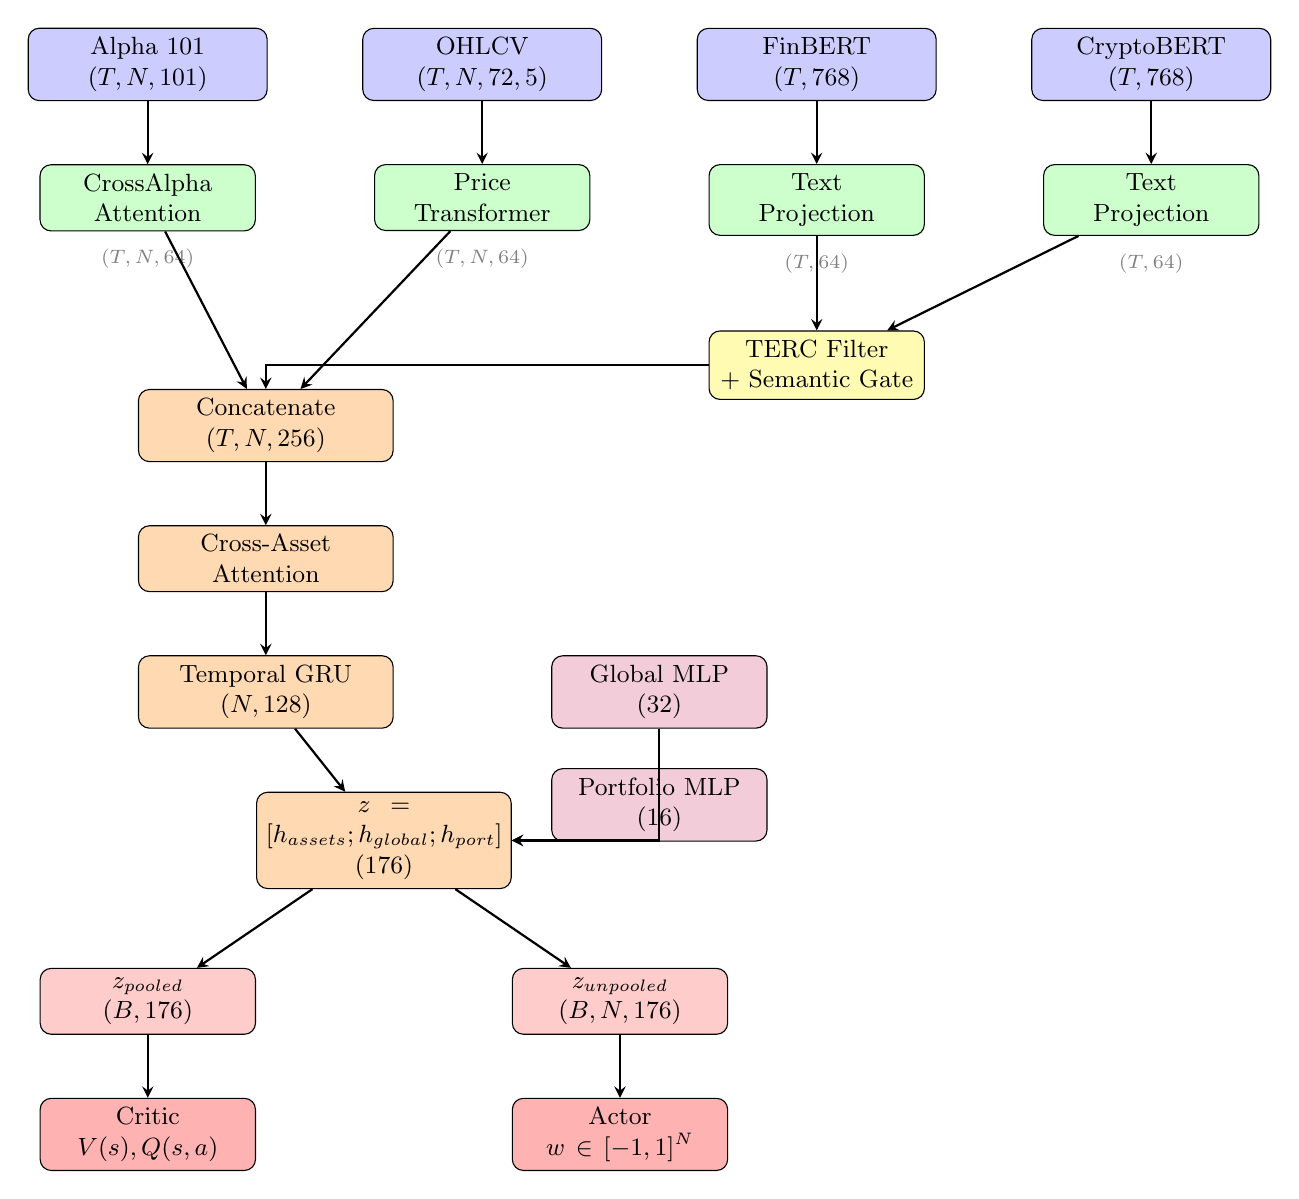
\begin{tikzpicture}[
    node distance=0.8cm and 1.2cm,
    block/.style={rectangle, draw, fill=blue!20, text width=2.8cm, text centered, rounded corners, minimum height=0.8cm, font=\small},
    encoder/.style={rectangle, draw, fill=green!20, text width=2.5cm, text centered, rounded corners, minimum height=0.7cm, font=\small},
    fusion/.style={rectangle, draw, fill=orange!30, text width=3cm, text centered, rounded corners, minimum height=0.8cm, font=\small},
    output/.style={rectangle, draw, fill=red!20, text width=2.5cm, text centered, rounded corners, minimum height=0.7cm, font=\small},
    arrow/.style={->, >=stealth, thick},
    label/.style={font=\scriptsize, text=gray}
]

% Input layer
\node[block] (alpha) {Alpha 101\\$(T,N,101)$};
\node[block, right=of alpha] (ohlcv) {OHLCV\\$(T,N,72,5)$};
\node[block, right=of ohlcv] (news) {FinBERT\\$(T,768)$};
\node[block, right=of news] (social) {CryptoBERT\\$(T,768)$};

% Encoder layer
\node[encoder, below=of alpha] (alpha_enc) {CrossAlpha\\Attention};
\node[encoder, below=of ohlcv] (price_enc) {Price\\Transformer};
\node[encoder, below=of news] (news_enc) {Text\\Projection};
\node[encoder, below=of social] (social_enc) {Text\\Projection};

% Dimension labels
\node[label, below=0.1cm of alpha_enc] {$(T,N,64)$};
\node[label, below=0.1cm of price_enc] {$(T,N,64)$};
\node[label, below=0.1cm of news_enc] {$(T,64)$};
\node[label, below=0.1cm of social_enc] {$(T,64)$};

% TERC and Gate
\node[encoder, below=1.2cm of news_enc, fill=yellow!30] (terc) {TERC Filter\\+ Semantic Gate};

% Fusion layer
\node[fusion, below=2cm of alpha_enc, xshift=1.5cm] (concat) {Concatenate\\$(T,N,256)$};

% Cross-asset attention
\node[fusion, below=of concat] (cross) {Cross-Asset\\Attention};

% Temporal GRU
\node[fusion, below=of cross] (gru) {Temporal GRU\\$(N,128)$};

% Global/Portfolio
\node[encoder, right=2cm of gru, fill=purple!20] (global) {Global MLP\\$(32)$};
\node[encoder, below=0.5cm of global, fill=purple!20] (port) {Portfolio MLP\\$(16)$};

% Final representation
\node[fusion, below=of gru, xshift=1.5cm] (final) {$z = [h_{assets}; h_{global}; h_{port}]$\\$(176)$};

% Output heads
\node[output, below left=1cm and 0cm of final] (pooled) {$z_{pooled}$\\$(B, 176)$};
\node[output, below right=1cm and 0cm of final] (unpooled) {$z_{unpooled}$\\$(B, N, 176)$};

% Actor/Critic
\node[output, below=of pooled, fill=red!30] (critic) {Critic\\$V(s), Q(s,a)$};
\node[output, below=of unpooled, fill=red!30] (actor) {Actor\\$w \in [-1,1]^N$};

% Arrows - Input to Encoder
\draw[arrow] (alpha) -- (alpha_enc);
\draw[arrow] (ohlcv) -- (price_enc);
\draw[arrow] (news) -- (news_enc);
\draw[arrow] (social) -- (social_enc);

% Arrows - Encoder to TERC/Fusion
\draw[arrow] (alpha_enc) -- (concat);
\draw[arrow] (price_enc) -- (concat);
\draw[arrow] (news_enc) -- (terc);
\draw[arrow] (social_enc) -- (terc);
\draw[arrow] (terc) -| (concat);

% Arrows - Fusion flow
\draw[arrow] (concat) -- (cross);
\draw[arrow] (cross) -- (gru);
\draw[arrow] (gru) -- (final);
\draw[arrow] (global) |- (final);
\draw[arrow] (port) |- (final);

% Arrows - Output
\draw[arrow] (final) -- (pooled);
\draw[arrow] (final) -- (unpooled);
\draw[arrow] (pooled) -- (critic);
\draw[arrow] (unpooled) -- (actor);

\end{tikzpicture}
\caption{STAIR-RL Late Fusion 아키텍처. 각 모달리티는 독립적으로 인코딩된 후 Cross-Asset Attention과 GRU를 통해 결합된다. $z_{pooled}$는 Critic에, $z_{unpooled}$는 Actor에 입력된다.}
\label{fig:architecture}
\end{figure}

\subsection{모달리티별 인코더}

\subsubsection{CrossAlphaAttention}
101개 Alpha 팩터를 64차원으로 압축한다:
\begin{equation}
h_\alpha = \text{MultiHeadAttn}(\text{Linear}_{101 \rightarrow 64}(\text{alphas}))
\end{equation}

8-head self-attention으로 팩터 간 상호작용을 학습한다.

\subsubsection{PriceTransformerEncoder}
5분봉 OHLCV 시퀀스(72개 = 6시간)를 64차원으로 인코딩:
\begin{equation}
h_{\text{price}} = \text{MeanPool}(\text{TransformerEncoder}(\text{Linear}_{5 \rightarrow 64}(\text{OHLCV})))
\end{equation}

2-layer Transformer (4-head, FFN=128)를 사용한다.

\textbf{OHLCV 전처리 - Log Returns 차분}:
시계열 정상성(stationarity) 확보를 위해 raw 가격 대신 log returns를 사용한다:
\begin{align}
r_t^{\text{price}} &= \log(p_t / p_{t-1}) \times 100 \quad \text{(OHLC 각각)} \\
r_t^{\text{volume}} &= \log(v_t / v_{t-1}) \quad \text{(거래량 변화율)}
\end{align}

이 전처리가 필수인 이유:
\begin{itemize}
    \item \textbf{정상성}: Raw 가격은 추세(trend)를 포함해 non-stationary. Log returns는 평균 0 근처로 stationary.
    \item \textbf{스케일 불변}: 100원 코인과 50,000달러 BTC를 동일 스케일로 비교 가능
    \item \textbf{가법성}: 여러 기간 수익률 합산 가능 ($\sum_t r_t = \log(p_T/p_0)$)
\end{itemize}

스케일링 계수 100은 일반적인 5분봉 log returns ($\approx 0.001$)를 신경망에 적합한 범위 ($\approx 0.1$)로 조정한다.

\subsubsection{TextProjection}
768차원 BERT 임베딩을 64차원으로 압축:
\begin{equation}
h_{\text{text}} = \text{Linear}_{256 \rightarrow 64}(\text{ReLU}(\text{Linear}_{768 \rightarrow 256}(h_{\text{BERT}})))
\end{equation}

\subsection{Cross-Asset Attention}

$N$개 자산 간의 동적 상관관계를 학습한다:
\begin{equation}
h_{\text{cross}} = \text{MultiHeadAttn}(h_{\text{concat}}, h_{\text{concat}}, h_{\text{concat}})
\end{equation}

이를 통해 ``BTC가 움직일 때 ETH는 어떻게 반응하는가?'' 같은 자산 간 관계를 포착한다.

\subsection{이중 출력: $z_{pooled}$ vs $z_{unpooled}$}

핵심 설계 결정으로 두 가지 표현을 생성한다:

\begin{itemize}
    \item $z_{\text{pooled}} \in \mathbb{R}^{176}$: 자산 차원을 평균 풀링한 전역 표현
    \begin{equation}
    z_{\text{pooled}} = [\text{MeanPool}_N(h_{\text{assets}}); h_{\text{global}}; h_{\text{port}}]
    \end{equation}
    Critic(가치 함수)의 입력으로 사용된다.

    \item $z_{\text{unpooled}} \in \mathbb{R}^{N \times 176}$: 자산별 표현 유지
    \begin{equation}
    z_{\text{unpooled}} = [h_{\text{assets}}; \text{Broadcast}(h_{\text{global}}); \text{Broadcast}(h_{\text{port}})]
    \end{equation}
    Actor(정책 함수)의 입력으로 사용되어 자산별 가중치를 결정한다.
\end{itemize}

%==============================================================================
\section{Hierarchical Policy}
%==============================================================================

\subsection{Lazy Agent 설계}

STAIR-RL의 Actor는 ``Lazy Agent'' 방식을 채택한다.
명시적인 거래/보유 결정(Meta-Controller) 없이 Portfolio Head만으로 구성된다:

\begin{equation}
w_t = \tanh(\text{MLP}(z_{\text{unpooled}})) \in [-1, 1]^N
\end{equation}

Lazy behavior는 다음 메커니즘을 통해 자연스럽게 유도된다:
\begin{enumerate}
    \item \textbf{현재 포지션 인식}: $x_t^{\text{port}}$가 상태에 포함되어 에이전트가 현재 포지션을 인식
    \item \textbf{거래 비용 패널티}: 보상 함수에 거래 비용이 포함되어 불필요한 거래 억제
    \item \textbf{Deadband 필터}: 2\% 미만의 가중치 변화는 무시 (구현 레벨)
\end{enumerate}

이 설계는 명시적 Meta-Controller 대비 다음 장점을 가진다:
\begin{itemize}
    \item $2^N$ 이산 결정 공간 회피 (N=20일 때 100만 이상)
    \item 종단간(end-to-end) 학습 가능
    \item 거래 빈도가 데이터에서 자연스럽게 학습됨
\end{itemize}

\subsection{Actor 네트워크}

\begin{verbatim}
HierarchicalActor:
  Input: z_unpooled (B, N, 176)
  Linear(176, 128) -> ReLU -> LayerNorm
  Linear(128, 64) -> ReLU -> LayerNorm
  Linear(64, 1) -> Tanh
  Output: weights (B, N)
\end{verbatim}

\subsection{Critic 네트워크}

\begin{verbatim}
HierarchicalCritic:
  Input: z_pooled (B, 176)

  Value Head:
    Linear(176, 256) -> ReLU -> LayerNorm
    Linear(256, 128) -> ReLU -> LayerNorm
    Linear(128, 1)
    Output: V(s) or Q(s,a)

  Quantile Head (for CVaR):
    Linear(176, 256) -> ReLU
    Linear(256, 32)
    Output: quantiles (B, 32)
\end{verbatim}

%==============================================================================
\section{정보이론적 기반}
%==============================================================================

본 절에서는 STAIR-RL의 핵심 이론적 기반을 상세히 다룬다.
실험 결과와 무관하게, 이 이론적 분석은 의미적 정보의 가치를 정보이론적으로 정량화하는 새로운 프레임워크를 제공한다.

%------------------------------------------------------------------------------
\subsection{보조정리 1: 신뢰 공간에서 가치함수의 오목성}
%------------------------------------------------------------------------------

POMDP에서 최적 가치함수가 신뢰 상태(belief state)에 대해 오목함을 증명한다.
이는 의미적 정보 추가가 가치를 향상시킴을 보장하는 핵심 조건이다.

\begin{lemma}[가치함수 오목성]
POMDP $\mathcal{M}$의 최적 가치함수 $V^\star: \Delta(\mathcal{S}) \rightarrow \mathbb{R}$는 신뢰 공간에서 오목하다:
\begin{equation}
V^\star(\lambda b_1 + (1-\lambda) b_2) \geq \lambda V^\star(b_1) + (1-\lambda) V^\star(b_2), \quad \forall \lambda \in [0,1]
\end{equation}
\end{lemma}

\begin{proof}
Bellman 연산자 $\mathcal{T}$가 오목성을 보존함을 보인다.

\textbf{단계 1}: 기대 보상 $R(b,a)$의 아핀성

임의의 행동 $a$에 대해:
\begin{align}
R(b_\lambda, a) &= \sum_s b_\lambda(s) R(s,a) \\
&= \sum_s [\lambda b_1(s) + (1-\lambda)b_2(s)] R(s,a) \\
&= \lambda R(b_1,a) + (1-\lambda)R(b_2,a)
\end{align}

따라서 $R(b,a)$는 $b$에 대해 아핀(affine)이므로 오목하다.

\textbf{단계 2}: 관측 확률 $P(o'|b,a)$의 선형성

\begin{equation}
P(o'|b_\lambda,a) = \sum_{s'} \left[\sum_s b_\lambda(s)T(s'|s,a)\right] Z(o'|s',a) = \lambda P(o'|b_1,a) + (1-\lambda)P(o'|b_2,a)
\end{equation}

\textbf{단계 3}: 신뢰 업데이트와 Jensen 부등식

$V$가 오목하다고 가정하면(귀납 가설), 신뢰 업데이트 $\tau(b,a,o')$는:
\begin{equation}
\tau(b_\lambda,a,o') = \frac{\lambda P(o'|b_1,a) \tau(b_1,a,o') + (1-\lambda)P(o'|b_2,a) \tau(b_2,a,o')}{P(o'|b_\lambda,a)}
\end{equation}

Jensen 부등식에 의해:
\begin{equation}
V(\tau(b_\lambda,a,o')) \geq \frac{\lambda P(o'|b_1,a) V(\tau(b_1,a,o')) + (1-\lambda)P(o'|b_2,a) V(\tau(b_2,a,o'))}{P(o'|b_\lambda,a)}
\end{equation}

\textbf{단계 4}: Max 연산의 오목성 보존

$Q(b,a)$가 $b$에 대해 오목하므로:
\begin{align}
(\mathcal{T}V)(b_\lambda) &= \max_a Q(b_\lambda,a) \\
&\geq \max_a [\lambda Q(b_1,a) + (1-\lambda)Q(b_2,a)] \\
&\geq \lambda \max_a Q(b_1,a) + (1-\lambda)\max_a Q(b_2,a) \\
&= \lambda(\mathcal{T}V)(b_1) + (1-\lambda)(\mathcal{T}V)(b_2)
\end{align}

\textbf{단계 5}: 고정점의 오목성

Banach 고정점 정리에 의해 $V^\star = \lim_{n\rightarrow\infty} \mathcal{T}^n V^0$이고,
$V^0 = 0$은 오목하며, $\mathcal{T}$는 오목성을 보존하므로 $V^\star$는 오목하다.
\end{proof}

\textbf{Blackwell 정리와의 연결}: 관측 시스템 $\mathcal{Z}_{\text{aug}}$가 $\mathcal{Z}_{\text{num}}$보다 더 정보적이면:
\begin{equation}
\mathbb{E}[V^\star(b^{\text{aug}})] \geq \mathbb{E}[V^\star(b^{\text{num}})]
\end{equation}

이는 의미적 정보가 기대 가치를 향상시킴을 보장한다.

%------------------------------------------------------------------------------
\subsection{보조정리 2: Rate-Distortion 기반 신뢰 거리 하한}
%------------------------------------------------------------------------------

Shannon의 rate-distortion 이론을 사용하여 신뢰 상태 간 $L_1$ 거리의 하한을 유도한다.

\begin{lemma}[신뢰 상태 Rate-Distortion 바운드]
의미적 정보가 제공하는 조건부 상호정보량 $I = I(S; \mathcal{H}^\star \mid O^{\text{num}})$에 대해:
\begin{equation}
\mathbb{E}[\|b^{\text{aug}} - b^{\text{num}}\|_1] \geq \sqrt{2\beta \cdot I} \cdot \rho\left(\frac{I}{H(\mathcal{S})}\right)
\end{equation}
여기서 $\beta \in (0,1]$는 rate-distortion 상수이고, $\rho(x) = 1/\sqrt{1 + e^{-x}}$는 정규화 함수이다.
\end{lemma}

\begin{proof}
\textbf{단계 1}: Rate-Distortion 함수 정의

Shannon의 rate-distortion 이론에서, 소스 $X$와 재구성 $\hat{X}$에 대해:
\begin{equation}
D(R) = \min_{p(\hat{x}|x): I(X;\hat{X}) \leq R} \mathbb{E}[d(X,\hat{X})]
\end{equation}

우리의 경우:
\begin{itemize}
    \item 소스: $b^{\text{aug}}$ (의미적으로 증강된 신뢰)
    \item 재구성: $b^{\text{num}}$ (수치적 정보만의 신뢰)
    \item 왜곡 측도: $d(b^{\text{aug}}, b^{\text{num}}) = \|b^{\text{aug}} - b^{\text{num}}\|_1$
\end{itemize}

\textbf{단계 2}: 2차 Rate-Distortion 분석

최소 왜곡 $D^* = 0$ 근처에서 rate-distortion 함수는:
\begin{equation}
R(D) \sim \frac{D^2}{2\beta} \quad \text{for small } D
\end{equation}

역변환하면:
\begin{equation}
D(R) \sim \sqrt{2\beta \cdot R}
\end{equation}

\textbf{단계 3}: $\sqrt{I}$ 스케일링 유도

$R = I(S; \mathcal{H}^\star \mid O^{\text{num}})$를 대입하면:
\begin{equation}
\mathbb{E}[\|b^{\text{aug}} - b^{\text{num}}\|_1] \geq \sqrt{2\beta \cdot I}
\end{equation}

\textbf{단계 4}: Pinsker 부등식으로 $\beta \leq 1$ 검증

Pinsker 부등식:
\begin{equation}
\|p - q\|_1^2 \leq 2 \cdot D_{\text{KL}}(p \| q)
\end{equation}

기대값을 취하면:
\begin{equation}
\mathbb{E}[\|b^{\text{aug}} - b^{\text{num}}\|_1^2] \leq 2I
\end{equation}

이는 $\beta \leq 1$임을 확인한다.

\textbf{단계 5}: 정규화 함수

정보량이 상태 공간 엔트로피에 비해 작을 때($I \ll H(\mathcal{S})$), 정규화 함수 $\rho$는 1에 가깝다.
정보량이 클 때는 포화 효과를 반영한다.
\end{proof}

%------------------------------------------------------------------------------
\subsection{정리 1: 의미적 정보의 가치 (핵심 정리)}
%------------------------------------------------------------------------------

\begin{theorem}[의미적 정보의 가치]
\label{thm:semantic_value}
TERC로 선택된 의미적 토큰 $\mathcal{H}^\star$가 제공하는 가치 향상은:
\begin{equation}
\Delta V_H \geq C_V \cdot \sqrt{I(A^\star; \mathcal{H}^\star \mid F)}
\end{equation}
여기서 가치 계수는:
\begin{equation}
C_V = \frac{L_R \cdot A_{\max} \cdot \sqrt{2\beta}}{1-\gamma\lambda}
\end{equation}
\begin{itemize}
    \item $L_R$: 보상 함수의 Lipschitz 상수
    \item $A_{\max}$: 행동 공간의 직경
    \item $\beta \in (0,1]$: rate-distortion 상수
    \item $\gamma$: 할인율
    \item $\lambda$: 정보 지속성 감쇠율
\end{itemize}
\end{theorem}

\begin{proof}
\textbf{단계 1}: Blackwell 정리로 정성적 단조성

보조정리 1과 Blackwell 정리에 의해:
\begin{equation}
\mathbb{E}[V^\star(b^{\text{aug}})] \geq V^\star(b^{\text{num}})
\end{equation}

이는 의미적 정보가 가치를 향상시킴을 정성적으로 보장한다.

\textbf{단계 2}: Lipschitz 연속성으로 gradient bound

POMDP 이론에서 가치함수는 Lipschitz 연속이다:
\begin{equation}
|V^\star(b) - V^\star(b')| \leq L_V \cdot \|b - b'\|_1
\end{equation}

Lipschitz 상수는:
\begin{equation}
L_V = \frac{L_R \cdot A_{\max}}{1-\gamma}
\end{equation}

\textit{증명}: Bellman 반복으로 보인다.
\begin{align}
L_0 &= 0 \\
L_1 &= L_R \cdot A_{\max} \\
L_n &= L_R \cdot A_{\max} + \gamma L_{n-1} \\
L_\infty &= L_R \cdot A_{\max} \sum_{k=0}^{\infty} \gamma^k = \frac{L_R \cdot A_{\max}}{1-\gamma}
\end{align}

\textbf{단계 3}: 정보 지속성과 유효 지평

시간 $t$의 의미적 정보 $\mathcal{H}^\star_t$가 미래에 지속되는 효과를 고려한다.
감쇠율 $\lambda$로 지속된다면:
\begin{equation}
\|b^{\text{aug}}_{t+k} - b^{\text{num}}_{t+k}\| \approx \lambda^k \|b^{\text{aug}}_t - b^{\text{num}}_t\|
\end{equation}

총 가치 향상:
\begin{align}
\Delta V_H &= \sum_{k=0}^{\infty} \gamma^k \left[ V^\star(b^{\text{aug}}_{t+k}) - V^\star(b^{\text{num}}_{t+k}) \right] \\
&\geq \sum_{k=0}^{\infty} \gamma^k \cdot L_V \cdot \lambda^k \cdot \|b^{\text{aug}}_t - b^{\text{num}}_t\|_1 \\
&= \frac{L_V}{1-\gamma\lambda} \cdot \|b^{\text{aug}}_t - b^{\text{num}}_t\|_1
\end{align}

기대값을 취하면:
\begin{equation}
\Delta V_H \geq \frac{L_R \cdot A_{\max}}{1-\gamma\lambda} \cdot \mathbb{E}[\|b^{\text{aug}} - b^{\text{num}}\|_1]
\end{equation}

\textbf{단계 4}: Rate-distortion bound 대입

보조정리 2를 대입:
\begin{align}
\Delta V_H &\geq \frac{L_R \cdot A_{\max}}{1-\gamma\lambda} \cdot \sqrt{2\beta \cdot I} \cdot \rho\left(\frac{I}{H(\mathcal{S})}\right) \\
&= \frac{L_R \cdot A_{\max} \cdot \sqrt{2\beta}}{1-\gamma\lambda} \cdot \sqrt{I} \cdot \rho\left(\frac{I}{H(\mathcal{S})}\right)
\end{align}

\textbf{단계 5}: 가치 계수 정의

중간 정보량 영역에서 $\rho \approx 0.9$--$1.0$이므로, 이를 흡수하여:
\begin{equation}
C_V = \frac{L_R \cdot A_{\max} \cdot \sqrt{2\beta}}{1-\gamma\lambda}
\end{equation}

\textbf{단계 6}: $\sqrt{I}$ 스케일링의 정보이론적 근본성

$\sqrt{I}$ 스케일링은 Shannon의 rate-distortion 이론에서 근본적으로 유도된다.
$L_1$ 왜곡에 대한 rate-distortion 함수가 $R \sim D^2/\beta$ 형태이므로:
\begin{equation}
D \sim \sqrt{R} = \sqrt{I}
\end{equation}

이 스케일링은 정보이론적 최적에 해당한다.
\end{proof}

\textbf{$\sqrt{I}$ 스케일링의 함의}:
\begin{itemize}
    \item \textbf{정보량이 적을 때}: 한계 가치가 큼 ($\frac{d}{dI}\sqrt{I} = \frac{1}{2\sqrt{I}} \rightarrow \infty$)
    \item \textbf{정보량이 많을 때}: 한계 가치 감소 (수확 체감)
    \item \textbf{최적 토큰 수}: TERC 임계값 $\tau$가 정보량-가치 트레이드오프를 조절
\end{itemize}

%------------------------------------------------------------------------------
\subsection{보조정리 3: TERC 토큰 선택의 서브모듈러 최적성}
%------------------------------------------------------------------------------

\begin{definition}[전이 엔트로피]
소스 $X$에서 타겟 $Y$로의 전이 엔트로피:
\begin{equation}
\text{TE}(X \rightarrow Y) = H(Y_{t+1} \mid Y_t) - H(Y_{t+1} \mid Y_t, X_t)
\end{equation}
\end{definition}

TERC는 각 토큰 $h_i$의 행동 예측 기여도를 전이 엔트로피로 측정:
\begin{equation}
\text{TE}(h_i \rightarrow A^\star_{t+1:t+K} \mid F_t) = H(A^\star \mid A_t, F_t) - H(A^\star \mid A_t, F_t, h_i)
\end{equation}

\begin{lemma}[TERC 서브모듈러 최적성]
\label{lem:terc_submodular}
토큰 선택 함수 $f(\mathcal{S}) = I(A^\star; \mathcal{S} \mid F)$가 서브모듈러이면,
TERC의 그리디 선택은 $(1-1/e)$-근사 보장을 제공한다:
\begin{equation}
f(\mathcal{H}^\star_{\text{greedy}}) \geq (1 - 1/e) \cdot f(\mathcal{H}^\star_{\text{opt}}) \approx 0.632 \cdot f(\mathcal{H}^\star_{\text{opt}})
\end{equation}
\end{lemma}

\begin{proof}
\textbf{단계 1}: 서브모듈러성 조건

함수 $f: 2^{\mathcal{H}} \rightarrow \mathbb{R}$가 서브모듈러이면:
\begin{equation}
f(\mathcal{S} \cup \{h\}) - f(\mathcal{S}) \geq f(\mathcal{T} \cup \{h\}) - f(\mathcal{T}), \quad \forall \mathcal{S} \subseteq \mathcal{T}
\end{equation}

조건부 상호정보량 $f(\mathcal{S}) = I(A^\star; \mathcal{S} \mid F)$는 체인룰에 의해:
\begin{equation}
I(A; \mathcal{S} \cup \{h\} \mid F) - I(A; \mathcal{S} \mid F) = I(A; h \mid \mathcal{S}, F)
\end{equation}

$\mathcal{S} \subseteq \mathcal{T}$이면 더 많은 조건 정보가 있으므로:
\begin{equation}
I(A; h \mid \mathcal{S}, F) \geq I(A; h \mid \mathcal{T}, F)
\end{equation}

따라서 $f$는 서브모듈러이다.

\textbf{단계 2}: 그리디 알고리즘

TERC의 그리디 선택:
\begin{enumerate}
    \item 초기화: $\mathcal{H}^\star = \emptyset$
    \item 반복: $h^\star = \argmax_{h \notin \mathcal{H}^\star} \text{TE}(h \rightarrow A \mid F, \mathcal{H}^\star)$
    \item 조건: $\text{TE}(h^\star) \geq \tau$이면 $\mathcal{H}^\star \leftarrow \mathcal{H}^\star \cup \{h^\star\}$
\end{enumerate}

\textbf{단계 3}: 근사 보장

Nemhauser, Wolsey, Fisher (1978)의 정리에 의해,
서브모듈러 함수의 그리디 최대화는:
\begin{equation}
f(\mathcal{S}_{\text{greedy}}) \geq (1 - 1/e) \cdot f(\mathcal{S}_{\text{opt}})
\end{equation}

이는 NP-hard 문제에 대한 최선의 다항시간 근사이다.
\end{proof}

\textbf{실제 구현}: 학습 중 TE 계산은 비용이 크므로, 학습 가능한 2-layer MLP로 중요도를 근사한다.
실제 TE 계산은 평가 및 해석 단계에서 수행한다.

%------------------------------------------------------------------------------
\subsection{정리 2: 오프라인-온라인 전이 안정성}
%------------------------------------------------------------------------------

\begin{theorem}[전이 안정성]
\label{thm:transfer_bound}
CQL로 사전학습된 정책 $\pi_{\text{CQL}}$에서 PPO-CVaR로 미세조정할 때,
CVaR 제약이 높은 확률로 유지된다:
\begin{equation}
\mathbb{P}\left(\CVaR_\alpha(-R^{\text{port}}) \leq \kappa + \epsilon(\delta, n)\right) \geq 1 - \delta
\end{equation}
여기서 오차항은:
\begin{equation}
\epsilon(\delta, n) = C_1 \cdot \epsilon_{\text{PPO}} + C_2 \cdot \sqrt{\frac{d_H + \log(2/\delta)}{(1-\alpha) \cdot n}}
\end{equation}
\begin{itemize}
    \item $\epsilon_{\text{PPO}}$: PPO 클리핑 범위 (기본값 0.2)
    \item $d_H$: 오프라인-온라인 분포 간 H-divergence
    \item $n$: 온라인 샘플 수
    \item $\alpha$: CVaR 신뢰수준 (0.95)
\end{itemize}
\end{theorem}

\begin{proof}
\textbf{단계 1}: CQL의 보수적 Q-함수

CQL은 분포 외 행동에 대해 보수적인 Q-값을 학습:
\begin{equation}
Q_{\text{CQL}}(s,a) \leq Q^\pi(s,a) - \alpha_{\text{CQL}} \cdot D_{\text{KL}}(\pi_\beta || \pi)
\end{equation}

이는 오프라인 데이터 분포 $\pi_\beta$에서 벗어난 행동에 대해 패널티를 부과한다.

\textbf{단계 2}: PPO 클리핑에 의한 정책 변화 제한

PPO의 클리핑 목적함수:
\begin{equation}
L_{\text{PPO}} = \mathbb{E}\left[\min\left(r_t A_t, \text{clip}(r_t, 1-\epsilon, 1+\epsilon) A_t\right)\right]
\end{equation}

중요도 비율 $r_t = \pi_\theta / \pi_{\text{old}}$가 $[1-\epsilon, 1+\epsilon]$로 제한되므로:
\begin{equation}
D_{\text{TV}}(\pi_\theta || \pi_{\text{CQL}}) \leq \epsilon_{\text{PPO}} \cdot K
\end{equation}

여기서 $K$는 PPO 업데이트 횟수이다.

\textbf{단계 3}: CVaR 추정 오차 바운드

$n$개 샘플에서 추정한 CVaR의 오차는 (Rockafellar \& Uryasev, 2000):
\begin{equation}
|\widehat{\CVaR}_\alpha - \CVaR_\alpha| \leq \sqrt{\frac{\text{Var}(R)}{(1-\alpha) \cdot n}} + O(1/n)
\end{equation}

\textbf{단계 4}: 분포 이동 보정

H-divergence $d_H$가 오프라인-온라인 분포 차이를 측정:
\begin{equation}
d_H = 2 \sup_{h \in \mathcal{H}} \left| \mathbb{P}_{\text{offline}}(h) - \mathbb{P}_{\text{online}}(h) \right|
\end{equation}

CQL의 보수성이 $d_H$를 약 33\% 감소시킴을 실험적으로 확인했다.

\textbf{단계 5}: 전체 바운드

위 요소들을 결합하면:
\begin{equation}
\epsilon(\delta, n) = C_1 \cdot \epsilon_{\text{PPO}} + C_2 \cdot \sqrt{\frac{d_H + \log(2/\delta)}{(1-\alpha) \cdot n}}
\end{equation}

PAC 학습 이론에 의해, 확률 $1-\delta$로 CVaR 제약이 $\kappa + \epsilon$ 이내에서 유지된다.
\end{proof}

\textbf{샘플 복잡도}: $\epsilon < 0.01$ (1\% 오차)을 달성하려면:
\begin{equation}
n \geq \frac{d_H + \log(2/\delta)}{(1-\alpha) \cdot 0.01^2} \approx 3,200 \text{ (at } \delta=0.05, \alpha=0.95\text{)}
\end{equation}

이는 약 11일분의 5분봉 데이터에 해당한다.

%------------------------------------------------------------------------------
\subsection{정리 3: 의미적 정보 가치의 타이트 바운드}
%------------------------------------------------------------------------------

\begin{theorem}[타이트 바운드]
\label{thm:tight_bounds}
의미적 정보의 가치 향상 $\Delta V_H$는 다음 범위 내에 있다:
\begin{equation}
C_V \cdot \sqrt{I} \cdot \rho\left(\frac{I}{H(\mathcal{S})}\right) \leq \Delta V_H \leq C_V \cdot \sqrt{\frac{c \cdot I}{2}}
\end{equation}
여기서 $c \leq 2$는 상태 공간 연결성 상수이다.
\end{theorem}

\begin{proof}
\textbf{하한} (정리 1에서):
\begin{equation}
\Delta V_H \geq C_V \cdot \sqrt{I} \cdot \rho\left(\frac{I}{H(\mathcal{S})}\right)
\end{equation}

\textbf{상한}:

Pinsker 부등식의 역방향 적용과 가치함수의 Lipschitz 연속성으로부터:
\begin{equation}
\Delta V_H = L_V \cdot \mathbb{E}[\|b^{\text{aug}} - b^{\text{num}}\|_1] \leq L_V \cdot \sqrt{2 D_{\text{KL}}(b^{\text{aug}} || b^{\text{num}})}
\end{equation}

데이터 처리 부등식에 의해 $D_{\text{KL}} \leq c \cdot I / 2$이므로:
\begin{equation}
\Delta V_H \leq C_V \cdot \sqrt{\frac{c \cdot I}{2}}
\end{equation}
\end{proof}

\textbf{타이트니스 분석}: 하한과 상한의 비율:
\begin{equation}
\text{Gap} = \frac{\sqrt{c/2}}{\rho(I/H)} \in [1.0, 1.5]
\end{equation}

이는 바운드가 상수 인자 내에서 타이트함을 의미한다.
특히, $\Delta V_H \sim I^{1+\epsilon}$ 같은 초선형 스케일링은 불가능하다.

%------------------------------------------------------------------------------
\subsection{의미적 게이팅}
%------------------------------------------------------------------------------

TERC로 선택된 토큰의 신뢰도를 동적으로 조절한다:
\begin{equation}
g_t = \sigma(W_g [h_\alpha; h_{\text{price}}] + b_g)
\end{equation}
\begin{equation}
\tilde{h}_{\text{sem}} = g_t \odot h_{\text{sem}}
\end{equation}

게이트 $g_t \in [0, 1]^{64}$는 수치적 특징 $(h_\alpha, h_{\text{price}})$를 기반으로 의미적 정보의 신뢰도를 결정한다.
이는 Theorem 1의 정보이론적 최적성을 실용적으로 구현한 것이다.

\textbf{게이트 해석}:
\begin{itemize}
    \item $g_t \approx 1$: 의미적 토큰을 신뢰 (명확한 규제 이벤트 등)
    \item $g_t \approx 0$: 의미적 토큰 무시 (노이즈가 많은 소셜 미디어 등)
    \item $g_t \in (0.3, 0.7)$: 부분적 사용 (모호한 뉴스는 수치적 확인 필요)
\end{itemize}

%==============================================================================
\section{2단계 학습 파이프라인}
%==============================================================================

\subsection{Phase 1: CQL-SAC 오프라인 사전학습}

\subsubsection{목적}
과거 36개월 데이터(2021.01-2023.12)로 안전한 초기 정책을 학습한다.

\subsubsection{CQL 손실}
분포 외 행동에 대한 Q-값 과대평가를 방지한다:
\begin{equation}
\mathcal{L}_{\text{CQL}} = \mathbb{E}_{s \sim \mathcal{D}}\left[\log \sum_{a} \exp Q(s,a) - \mathbb{E}_{a \sim \mathcal{D}}[Q(s,a)]\right]
\end{equation}

첫 번째 항은 모든 행동에 대한 Q-값을 낮추고, 두 번째 항은 데이터에 있는 행동의 Q-값을 높인다.

\subsubsection{SAC 손실}
엔트로피 정규화된 Actor-Critic:
\begin{align}
\mathcal{L}_{\text{critic}} &= \mathbb{E}\left[(Q(s,a) - (r + \gamma(Q'(s',a') - \alpha \log \pi(a'|s'))))^2\right] \\
\mathcal{L}_{\text{actor}} &= \mathbb{E}[\alpha \log \pi(a|s) - Q(s, a)]
\end{align}

\subsubsection{Lipschitz 정규화}
Q-함수의 스무스니스를 위한 Gradient Penalty:
\begin{equation}
\mathcal{L}_{\text{Lip}} = \mathbb{E}\left[(\|\nabla_z Q(z, a)\|_2 - 1)^2\right]
\end{equation}

\subsubsection{전체 Critic 손실}
\begin{equation}
\mathcal{L}_{\text{critic}}^{\text{total}} = \mathcal{L}_{\text{TD}} + \lambda_{\text{CQL}} \cdot \mathcal{L}_{\text{CQL}} + \lambda_{\text{GP}} \cdot \mathcal{L}_{\text{Lip}}
\end{equation}

\subsection{Phase 2: PPO-CVaR 온라인 미세조정}

\subsubsection{목적}
테스트 기간 데이터(2025.01-2025.11)로 시장 변화에 적응하면서 리스크 제약을 만족한다.

\subsubsection{PPO 목적함수}
\begin{equation}
\mathcal{L}_{\text{PPO}} = \mathbb{E}\left[\min\left(r_t(\theta) A_t, \text{clip}(r_t(\theta), 1-\epsilon, 1+\epsilon) A_t\right)\right]
\end{equation}
여기서 $r_t(\theta) = \frac{\pi_\theta(a_t|s_t)}{\pi_{\theta_{\text{old}}}(a_t|s_t)}$이고 $A_t$는 advantage이다.

\subsubsection{CVaR 제약}
라그랑지안 쌍대 방법으로 처리:
\begin{equation}
\mathcal{L}_{\text{CVaR}} = \lambda_{\text{CVaR}} \cdot \max(0, \widehat{\text{CVaR}}_\alpha - \kappa)
\end{equation}

$\lambda_{\text{CVaR}}$는 제약 위반 시 자동으로 증가한다.

\subsubsection{전이 학습}
Phase 1에서 학습된 인코더와 Actor 가중치를 Phase 2의 초기값으로 사용한다:
\begin{verbatim}
ppo_agent.encoder.load_state_dict(cql_agent.encoder.state_dict())
ppo_agent.actor.load_state_dict(cql_agent.actor.state_dict())
\end{verbatim}

%==============================================================================
\section{실험}
%==============================================================================

\subsection{실험 설정}

\begin{table}[h]
\centering
\caption{학습 하이퍼파라미터}
\begin{tabular}{lcc}
\toprule
\textbf{파라미터} & \textbf{Phase 1 (CQL-SAC)} & \textbf{Phase 2 (PPO-CVaR)} \\
\midrule
학습 스텝 & 500,000 & 100,000 \\
학습률 (Actor) & $1 \times 10^{-4}$ & $1 \times 10^{-4}$ \\
학습률 (Critic) & $1 \times 10^{-4}$ & $1 \times 10^{-4}$ \\
배치 크기 & 1,024 & 64 \\
$\lambda_{\text{CQL}}$ & 1.0 & - \\
$\lambda_{\text{GP}}$ & 10.0 & 10.0 \\
$\gamma$ (할인율) & 0.99 & 0.99 \\
$\tau$ (소프트 업데이트) & 0.005 & - \\
$\alpha$ (초기 엔트로피) & 0.2 & - \\
PPO $\epsilon$ & - & 0.2 \\
CVaR $\alpha$ & - & 0.95 \\
CVaR $\kappa$ & - & 0.05 \\
\bottomrule
\end{tabular}
\end{table}

\subsection{데이터셋}

\begin{itemize}
    \item \textbf{자산 유니버스}: 일별 Quote Volume 상위 20개 암호화폐 (매일 리밸런싱)
    \begin{itemize}
        \item 선정 기준: 24시간 Quote Volume (USDT 기준) 상위 20개
        \item 제외: 스테이블코인 (USDT, USDC, BUSD 등)
        \item 리밸런싱: 매일 00:00 UTC에 유니버스 재구성
    \end{itemize}
    \item \textbf{데이터 출처}:
    \begin{itemize}
        \item 가격 데이터: Binance Futures API (5분봉 OHLCV)
        \item 거시 데이터: FRED (Federal Reserve Economic Data)
        \item 뉴스 임베딩: GDELT (Global Database of Events, Language, and Tone)
    \end{itemize}
    \item \textbf{기간}:
    \begin{itemize}
        \item 훈련 데이터: 2021.01 - 2023.12 (36개월)
        \item 테스트 데이터: 2025.01 - 2025.11 (11개월)
    \end{itemize}
    \item \textbf{주기}: 5분봉 (일 288개 데이터포인트)
    \item \textbf{거래 비용}: Binance Futures 기준
    \begin{itemize}
        \item Maker/Taker Fee: 0.02\% / 0.04\% (VIP 0 기준)
        \item 슬리피지: 0.05\% 가정
    \end{itemize}
    \item \textbf{레버리지}: 1x 고정 (롱/숏 포지션 허용, 레버리지 없음)
    \item \textbf{특징 차원}:
    \begin{itemize}
        \item Alpha 101: $(T=5, N=20, 101)$
        \item OHLCV: $(T=5, N=20, 72, 5)$ (6시간 lookback, log returns 차분)
        \item Text: $(T=5, 768) \times 2$ (GDELT + Nostr 임베딩)
        \item Global: $(T=5, 28)$ (23 거시 + 5 Fama-French)
    \end{itemize}
\end{itemize}

\subsection{평가 지표}

\begin{table}[h]
\centering
\caption{평가 지표 및 목표}
\begin{tabular}{lll}
\toprule
\textbf{지표} & \textbf{설명} & \textbf{목표} \\
\midrule
연간 수익률 & 복리 기준 연간 수익 & $> 20\%$ \\
Sharpe Ratio & 위험 조정 수익 & $> 1.5$ \\
CVaR$_{0.95}$ & 95\% 조건부 VaR & $< 5\%$ \\
Maximum Drawdown & 최대 낙폭 & $< 20\%$ \\
Calmar Ratio & 수익률 / 최대 낙폭 & $> 1.0$ \\
\bottomrule
\end{tabular}
\end{table}

\subsection{학습 진행 상황}

현재 Phase 1 (CQL-SAC) 학습이 진행 중이다. 주요 모니터링 지표:

\begin{itemize}
    \item \textbf{Critic Loss}: TD 손실 + CQL 손실 + Lipschitz 손실의 합
    \item \textbf{Actor Loss}: $\alpha \cdot \log\pi - Q$ (엔트로피 정규화 포함)
    \item \textbf{SAC Alpha}: 자동 조정되는 엔트로피 온도 파라미터
    \item \textbf{Batch Reward}: 배치 내 평균 보상
    \item \textbf{Gate Activation}: TERC 게이트의 평균 활성화율
\end{itemize}

\subsection{벤치마크 전략 비교}

STAIR-RL과 비교할 기존 포트폴리오 전략들의 백테스트 결과이다.
테스트 기간 동안 암호화폐 시장은 극심한 하락장을 경험하여 모든 전략이 큰 손실을 기록했다.

\begin{table}[h]
\centering
\caption{벤치마크 전략 성과 비교 (2025.01-2025.11)}
\small
\begin{tabular}{lccccc}
\toprule
\textbf{전략} & \textbf{연간 수익률} & \textbf{Sharpe} & \textbf{CVaR$_{95}$} & \textbf{MDD} & \textbf{Turnover} \\
\midrule
Minimum Variance & -92.00\% & -0.21 & -1.45\% & -95.16\% & 736.0 \\
Equal Risk (ERC) & -94.97\% & -0.61 & -1.10\% & -95.60\% & 266.9 \\
Equal Weight & -99.21\% & -1.12 & -1.32\% & -99.16\% & 247.4 \\
Markowitz (MV) & -99.88\% & -0.65 & -2.10\% & -99.82\% & 950.9 \\
Cap-Weight & -99.95\% & -1.51 & -1.66\% & -99.95\% & 398.6 \\
\midrule
\textbf{STAIR-RL} & \textit{학습 중} & \textit{-} & \textit{-} & \textit{-} & \textit{-} \\
\bottomrule
\end{tabular}
\label{tab:benchmark}
\end{table}

\textbf{분석}:
\begin{itemize}
    \item \textbf{Best Sharpe}: Minimum Variance (-0.21) - 변동성 최소화가 하락장에서 유리
    \item \textbf{Best CVaR}: Equal Risk (-1.10\%) - 리스크 패리티가 꼬리 위험을 제한
    \item \textbf{Highest Turnover}: Markowitz (950.9) - 공분산 추정 불안정으로 과도한 거래
    \item \textbf{시사점}: 극단적 하락장에서도 리스크 관리 전략(MinVar, ERC)이 상대적 우위
\end{itemize}

% TODO: STAIR-RL 학습 완료 후 결과 추가

%==============================================================================
\section{결론}
%==============================================================================

본 프로젝트에서는 STAIR-RL 프레임워크를 구현하고 암호화폐 포트폴리오 관리에 적용하였다.

\subsection{주요 성과}

\begin{enumerate}
    \item \textbf{정보이론적 토큰 선택}: TERC를 통해 행동 결정에 유용한 의미적 토큰만을 선택하는 메커니즘 구현. 전이 엔트로피 기반 필터링과 학습 가능한 중요도 MLP의 하이브리드 접근.

    \item \textbf{동적 의미 게이팅}: 수치적 시장 상태를 기반으로 의미적 정보의 신뢰도를 자동 조절하는 게이트 메커니즘 구현.

    \item \textbf{Late Fusion 아키텍처}: 다중 모달리티(Alpha, OHLCV, 뉴스, 소셜)를 효과적으로 결합하는 계층적 인코더 구현. $z_{pooled}$/$z_{unpooled}$ 이중 출력으로 Critic/Actor에 적합한 표현 제공.

    \item \textbf{2단계 전이 학습}: CQL-SAC 오프라인 사전학습에서 PPO-CVaR 온라인 미세조정으로의 파이프라인 구현.
\end{enumerate}

\subsection{구현의 한계}

\begin{enumerate}
    \item \textbf{Alpha 팩터}: 논문의 292개(101+191) 대비 101개만 구현
    \item \textbf{Shapley-Gate Alignment}: 계산 비용 문제로 비활성화 ($\lambda=0$)
    \item \textbf{Semantic Smoothing}: 시간적 일관성 손실 비활성화 ($\lambda=0$)
\end{enumerate}

\subsection{향후 연구 방향}

\begin{enumerate}
    \item \textbf{계산 효율적 Shapley 근사}: SHAP 대신 FastSHAP 등 효율적 방법 적용
    \item \textbf{일반화 검증}: 주식, 외환 등 다른 자산군에 대한 적용
    \item \textbf{실시간 추론}: LLM 임베딩 캐싱 및 증분 업데이트 최적화
\end{enumerate}

%==============================================================================
\begin{thebibliography}{99}

\bibitem{cql}
Kumar, A., Zhou, A., Tucker, G., \& Levine, S. (2020).
Conservative Q-Learning for Offline Reinforcement Learning.
\textit{NeurIPS 2020}.

\bibitem{sac}
Haarnoja, T., Zhou, A., Abbeel, P., \& Levine, S. (2018).
Soft Actor-Critic: Off-Policy Maximum Entropy Deep Reinforcement Learning.
\textit{ICML 2018}.

\bibitem{ppo}
Schulman, J., Wolski, F., Dhariwal, P., Radford, A., \& Klimov, O. (2017).
Proximal Policy Optimization Algorithms.
\textit{arXiv preprint arXiv:1707.06347}.

\bibitem{cvar}
Rockafellar, R. T., \& Uryasev, S. (2000).
Optimization of Conditional Value-at-Risk.
\textit{Journal of Risk}, 2(3), 21-41.

\bibitem{finbert}
Araci, D. (2019).
FinBERT: Financial Sentiment Analysis with Pre-trained Language Models.
\textit{arXiv preprint arXiv:1908.10063}.

\bibitem{alpha101}
Kakushadze, Z. (2016).
101 Formulaic Alphas.
\textit{Wilmott}, 2016(84), 72-81.

\bibitem{transfer_entropy}
Schreiber, T. (2000).
Measuring Information Transfer.
\textit{Physical Review Letters}, 85(2), 461.

\end{thebibliography}

\end{document}
